
\documentclass[12pt,a4]{article}
%%%%%%%%%%%%%%%%%%%%%%%%%%%%%%%%%%%%%%%%%%%%%%%%%%%%%%%%%%%%%%%%%%%%%%
\usepackage{amsmath,amsthm}
\usepackage{bm}
\usepackage{amsfonts}
\usepackage{amssymb}
\usepackage[normalem]{ulem}
\usepackage{enumerate}
\usepackage{graphicx}%
\usepackage{datetime,verbatim}
\usepackage{cite}
\usepackage{hyperref} 
\usepackage{listings}

%%%%%%%%%%%%%%%%%%%%%    page setup   %%%%%%%%%%%%%%%%%%%%%%%%%%%%%%% 

\textheight=245truemm \textwidth=160truemm \hoffset=-8truemm
\voffset=-23truemm

%%%%%%%%%%%%%%%%%%%%%%%%%%%%%%%%%%%%%%%%%%%%%%%%%%%%%%%%%%%%%%%%%%%%%
\usepackage{fancyhdr}
\pagestyle{fancy}
\lhead{{\sf\scriptsize }}
\rhead{{\sf\scriptsize Winter~2020}}
\chead{{\sf\scriptsize Linear Algebra: Course Project @  DS master programme at UCU}}

\lfoot{}
\rfoot{}
\cfoot{\rm\thepage}

%%%%%%%%%%%%%%%%%%%%%%%%%%%%%%%%%%%%%%%%%%%%%%%%%%%%%%%%%%%%%%%%%%%%%


%%%%%%%%%%%%%%%%%%%%%%%%%%%%%%%%%%%%%%%%%%%%%%%%%%%%%%%%%%%%%%%%%%%%%


%%%%%%%%%%%%%%%   matrix extension  %%%%%%%%
\makeatletter
\renewcommand*\env@matrix[1][*\c@MaxMatrixCols c]{%
	\hskip -\arraycolsep
	\let\@ifnextchar\new@ifnextchar
	\array{#1}}
\makeatother
%%%%%%%%%%%%%%%%%%%%%%%%%%%%%%%%%%%%%%%%%%%%

\newenvironment{proofNoQED}[1]{\smallskip\noindent{\it Proof #1.}\ \rm}
{\hfill \smallskip}
\newcommand{\ProofNoQED}[1]{\smallskip\noindent{\it Proof} #1\ \hfill\smallskip}
%\renewcommand{\qedsymbol}{\text{$\square$}}

\newtheorem{problem}{Problem}

%%%%%%%%%%%%%%%%%%%%%%%%%%%%%%%%%%%%%%%%%%%%%%%%%%%%%%%%%%%%%%%%%%%%%

%%%%%%%%%%%%%%%%%%%%%%%%%%%%%   Definitions       %%%%%%%

\newcommand\ls{\operatorname{ls}}
\newcommand\rank{\operatorname{rank}}
\newcommand{\trace}{\operatorname{tr}}
\newcommand\grad{\operatorname{grad}}


\newcommand{\ov}{\overline}
\newcommand{\wt}{\widetilde}

\newcommand{\bla}{\bm{\lambda}}


\newcommand{\bN}{{\mathbb N}}
\newcommand{\bR}{{\mathbb R}}
\newcommand{\bZ}{{\mathbb Z}}

\newcommand{\ba}{{\mathbf a}}
\newcommand{\bb}{{\mathbf b}}
\newcommand{\bff}{{\mathbf f}}

\newcommand{\bu}{{\mathbf u}}
\newcommand{\bv}{{\mathbf v}}
\newcommand{\bp}{{\mathbf p}}
\newcommand{\bq}{{\mathbf q}}
\newcommand{\br}{{\mathbf r}}
\newcommand{\bx}{{\mathbf x}}
\newcommand{\by}{{\mathbf y}}
\newcommand{\bw}{{\mathbf w}}

\newcommand{\cB}{{\mathcal B}}
\newcommand{\cF}{{\mathcal F}}
\newcommand{\cG}{{\mathcal G}}
\newcommand{\cN}{{\mathcal N}}
\newcommand{\cP}{{\mathcal P}}
\newcommand{\cT}{{\mathcal T}}

%%%%%%%%%%%%%%%%%%%%%%%%%%%%%%%%%%%%%%%%%%%%%%%%%%%%%%%%%%%%%%%%%%%%%


\begin{document}

\begin{center}
  \Huge\bf{Keystroke Dynamics in User Identification}
\end{center}

\begin{center}
	Sevil Smailova, Kateryna Ruskykh and Volodymyr Byno
\end{center}

\large\textbf{Abstract}
\bigskip

\normalsize
In this course project, we will study keystroke dynamics as a method to authenticate people in online assessment situations. We will review the theory behind keystroke dynamics: why this method is useful, what math is inside the key approaches to keystroke analysis if this method works or not based on the findings of other researchers. In the practical part, we will run the keystroke analysis (its simplified version) on a large existing dataset to verify if this method works. We will also attempt to create our own small dataset of keystroke prints of our groupmates/acquaintances and test if our algorithm will work fine and will be able to identify people correctly. 
\bigskip

\large\textbf{Introduction}
\bigskip

\normalsize
Keystroke dynamics is a method to identify people using their typing patterns that is especially relevant for the tasks of online identity verification. While physiological biometrics (finger scan, iris scan, retina scan, hand scan, and facial scan) give very good precision, these methods are quite costly. Keystroke dynamics is less costly and a relatively accurate method to use by online education institutions. 

Keystroke Dynamics is now widely used in a variety of areas:

\begin{itemize}
	\item Authentication: Typing pattern can be used as an additional step in an authentication flow, to double-check if the password is being entered by the same person.
	\item Online education platforms: there is a growing need to recognize actual and reduce potential cheating of students. Cheating and manipulations must be eliminated to certify students and prove their competence. 
	\item Marketing: The sites could build their marketing strategy based on the visitors' typing patterns. With the high rate of probability, they can create a user's profile based on typing patterns and display relevant advertisements even before the user actually creates a profile. 
	\item Fraud detection: Keystroke dynamics can help identify attackers even though they are anonymous. They can be detected without even being authenticated.
	\item The detection of emotions: stress, calmness, anger could be detected thanks to the analysis of the way a user types the messages. 
	\item Bank Security: In 2005, the Bank of Ireland added the keystroke dynamics algorithms to the user's authentication process. Since then keystroke dynamics became very popular among banks. Ecuador bank, Bank of Utah, and others use it in their authentication systems.
\end{itemize}	

In addition to the items above, the keystroke dynamics market \href{https://findbiometrics.com/amr-forecasts-booming-keystroke-dynamics-market/}{is expected to grow in the nearest future}.

There are a multiple typing patterns that can be measured and analyzed in a keystroke dynamics: an amount of time a key is depressed, time between a previous key is down and next key is up, typing speed (the average number of keystrokes), overlapping of some key combinations, number of errors, while typing and so on. To track the patterns a keystroke digraph latency time is used: the time that lapses between the stroke of two adjacent letters. 

Keystroke dynamics is not static: it can change as skills of a typing person increase or her health status is changed (for instance, finger injury). This requires re-collecting and updating typing datasets, which is relatively inexpensive. Data scientists can gather much additional information: typing patterns, when a person is standing or sitting, when her finger is injured, when she is coping some text or in opposite prints freely, etc. In our project, we will analyze basic typing patterns to simplify our work, although the precision will certainly be smaller.

\bigskip

\large\textbf{Literature Review}
\bigskip

\normalsize
The earliest start of significant keystroke dynamics (KD) research dates back to late 1970s and early 1980s \cite{Teh:2013}, \cite{Liakat:2017}, \cite{killourhy2009comparing}. After 2003 the number of papers on KD increased significantly, indicating a high interest in the topic \cite{Teh:2013}. Indeed, google scholar returns 62 publications on KD in 2000, 103 in 2003, 232 in 2005 and 995 in 2019, implying a 16 times boost in number of publications between 2000 and 2019. The research on KD varies a lot in their topics (verification vs identification), platform (desktop vs mobile/ tablet), data-collection strategies (size, input type), feature sets, static or dynamic character etc.

The KD publications that focus on verification (the process of proving a validity of claimed identity) outnumber identification (the processes of recognizing a presented identity), as the latter is time-consuming and requires more processing capacities \cite{Teh:2013}, \cite{banerjee2014_emnlp}. Most of the publications on KD do their research on a relatively small dataset involving 21-50 people, typically scholars or students from the researchers’ institution capacities [1,6]. According to the research of 2016, 40 \% out of 88 of the KD publications reviewed involved 21-50 participants, while the reviews of up to 20 and over 100 people accounted for 24 \% each \cite{Liakat:2017}. In recent years KD researchers have more opportunities to expand the number of participants involved and size of collected datasets.

The KD research can deal with a short-text input (password, username, short text phrase, digits) or long-text (over 100 words). The latter can be unconstrained free-text that is often used in continuous authentication systems - systems that dynamically check users’ identities while they are typing. In the review of 2016 the short-text and digits publications account for 60 \% out of 88, while long-text publications take a 22 \% share \cite{Liakat:2017}.

The most common features that are used in the KD research are timing measures: dwell time (the time interval between press of a key and its release) and flight time (the time interval between releasing one key and pressing the other). Most of the researchers use di-graphs: timing measures between two consecutive keys, but n-graphs (three or more keys) can be also used). Other features used by researchers are mouse position / movement, pressure, text correction features, frequencies of errors, average typing speed / acceleration, etc.

There are also a variety of methods to analyze keystroke data that can be grouped as statistical methods (mean, deviations, t-tests, outlier count (z-score), chi-squared, Bayesian modelling, logistic regression, etc.), distance measures (Euclidean, Manhattan, Mahalanobis, Chebyshev, other distance-based measures) and machine learning methods (Artificial Neural Networks, decision trees, KNN, random forest, SVM, etc.). However, it is hard to compare performance and accuracy metrics of different methods, as different authors use different databases, sets of features, model parameters, input types, modes (static or dynamic), etc. There is a benchmark research of Killourhy and Maxion that dates back to 2009, where the authors collect (and make it public) a dataset and compare 14 different methods (detectors) in similar settings \cite{killourhy2009comparing}.

Killourhy and Maxion selected  a 10-character password “.tie5Roanl” , recruited 51 people who were asked to type the password 400 times in 8 sessions. The feature set used included  Keydown-Keydown time between consecutive keys (in some publications referred to as latency), dwell time and flight time. And the authors used 14 algorithms (detectors) that had produced promising results in research of other scientists for authentication of potential impostors. The best-performing algorithms are defined, using two metrics: equal-error rate / ERR (a threshold to discriminate a potential impostor is chosen to have equal miss and false alarm rates) and zero-miss false-alarm rate / ZMFAR (a threshold is selected in a way that a miss rate is 0 and false alarm rate is minimized). We list the top 5 using these 2 metrics in the table below:

\begin{center}

\begin{tabular*}{\textwidth}{l @{\extracolsep{\fill}} lllll}

\hline
 & \textbf{Detector} & \textbf{EER} & & \textbf{Detector} & \textbf{ZMFAR} \\
 \hline
1. & Manhattan (scaled) & 0.096 & 1. & Nearest Neighbor (Mahalanobis) & 0.468 \\ 
\hline
2. & Nearest Neighbor (Mahalanobis) & 0.100 & 2. & Mahalanobis & 0.482 \\ 
\hline
3. & Outlier Count (z-score) & 0.102 & 3. & Mahalanobis (normed) & 0.482 \\

\hline
4. & SVM (one-class) & 0.102 & 4. & SVM (one-class) & 0.504 \\
\hline
5. & Mahalanobis & 0.110 & 5. & Manhattan (scaled) & 0.601 \\
\hline
\end{tabular*}
\caption{\textbf{Table 1:} The best algorithms / detectors for KD authentication by Killourhy and Maxion}
\end{center}

Interestingly, the simplest distance algorithms show the best results according to Killourhy and Maxion. There is also a good score for a machine learning SVM detector and a statistical z-score method. Neural Networks (standard) and k-means give the worst results out of 14 algorithms tested.

Other researchers have been questioning the results of Killourhy and Maxion, testing algorithms on different text inputs (long-text) and datasets (unconstrained datasets of free text). Overall, statistical and distance methods have been losing popularity, while machine learning approaches are gaining pace in the modern times \cite{Liakat:2017}. Support Vector Machine (SVM) is  considered by some researchers as a prevailing machine learning classification approach that produces good results and has reasonable complexity \cite{Liakat:2017}, \cite{raul2020comprehensive}.

\bigskip
\large\textbf{Sketch of the possible approaches }
\bigskip

\normalsize
To analyze password-typing data we need a feature set that is contained from main metrics that measure the typing rhythm and the anomaly detection algorithm that measures the percentage of impostor passwords that are not detected and percentage of genuine user passwords that are mistakenly detected as impostors.  

The classic anomaly-detection algorithm \cite{duda2001_patternClass} models each password as a point in p-dimensional space, where p - is the number of features in the timing vectors. It treats the training data as a cloud of points and computes the anomaly score of the test vector based on its proximity to the center of this cloud. Specifically, in the training phase, the mean vector of the set of timing vectors is calculated. In the test phase, the anomaly score is calculated as the squared Euclidean distance between the test vector and the mean vector.

There are a lot of modifications of measuring the distance between the test vector and the mean vector: distance can be normalized and scaled, as a distance can be taken the Manhattan or Mahalanobis distance. 
The are other approaches in evaluating the anomaly score. The nearest-neighbor algorithm solves a classification problem using the mentioned distances. A neural network can reproduce the input feature vector as the output or simply calculate the anomaly score on the output layer. To detect the anomaly score, the fuzzy algorithm can be used. The key idea is that the ranges of typing times are assigned to fuzzy sets. The sets are called fuzzy because elements can partially belong to a set. In the training phase, the detector determines how strongly each feature belongs to each set, and each feature is matched with the set in which its membership is strongest. In the test phase, each timing feature is checked to see if it belongs to the same set as the training data. The anomaly score is calculated as the average lack of membership across all test vector timing features. SVM algorithms project the data from a single class and find a separator between the projection and the origin.

\newpage
\bigskip
\large\textbf{Short explanations of the pros and cons of your chosen method}
\bigskip

\normalsize
We will try to implement the classification KNN algorithm.\\
Pros:
\begin{itemize}
    \item pretty simple to interpret;
    \item a good algorithm to model nonlinear data. 
\end{itemize}


Cons:
\begin{itemize}
    \item computationally expensive. 
\end{itemize}



\bigskip
\large\textbf{Dataset}
\bigskip

\normalsize
There are some datasets containing repeated data, but they are too small for the task. For example, the dataset containing the same passwords inputted by 50 different users might be good for the baseline test of the proof of concept, but it is not enough to achieve any robust judgments.
We have chosen the  \href{http://www3.cs.stonybrook.edu/~rbanerjee/project-pages/keystrokes/keystrokes.html}{Keystroke Patterns as Prosody in Digital Writings} dataset \cite{banerjee2014_emnlp}. It contains of 3 datasets: \begin{itemize}
	\item \textbf{Restaurant Reviews}: The dataset consists of 1000 unique restoran reviews inputed by 500 unique users
	\item \textbf{Gun Control}: The dataset consists of 800 unique essays on "Gun Control" from 400 unique users
	\item \textbf{Gay Marriage}: The dataset consists of 800 unique essays on "Gay Merriage" topic  from 400 unique users
\end{itemize}

The typical raw data in the dataset looks like this:
\bigskip

\begin{text}
	0 MouseUp 0 0;16705 KeyDown 16;17170 KeyDown 16;17200 KeyDown 16;17229 KeyDown 16;17258 KeyDown 16;17287 KeyDown 16;17317 KeyDown 16;17346 KeyDown 16;17375 KeyDown 16;17404 KeyDown 16;17433 KeyDown 16;17463 KeyDown 16;17492 KeyDown 16; ...
\end{text}

Providing the preprocessing and cleaning steps, we've obtained the transition time (latency between key presses) and dwell time (the amount of time a key is depressed) for each of the users' keystrokes.

Lets take a look at the transition time distribution in "Restaurant Reviews" dataset:
\begin{center}
\centering
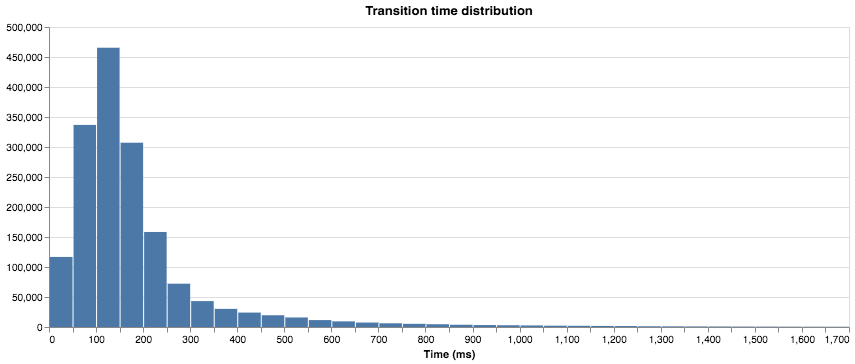
\includegraphics[width=0.85\linewidth]{images/transitions_time.png}
\end{center}

and dwell time distribution:

\begin{center}
	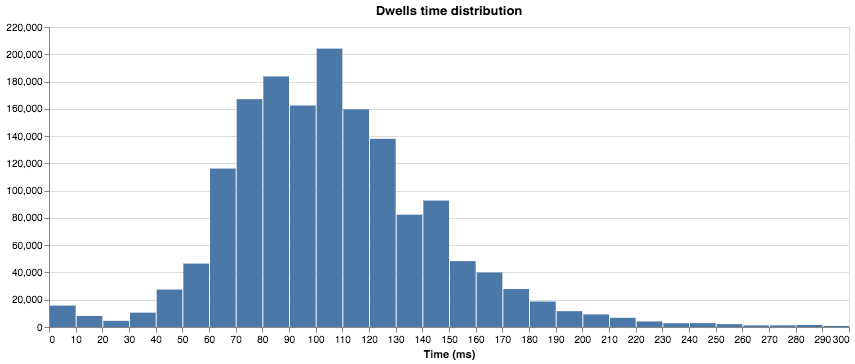
\includegraphics[width=0.85\linewidth]{images/dwells_time.png}
	\label{fig:transitions_time.png}
\end{center}

As we see, both distributions are close to normal. They also do not deverge a lot from the distributions obtained in Richards Young dissertation \cite{richards_young_2018}.
We also filered out the characters that had too low occurency number.

\bigskip
\large\textbf{Future steps}
\bigskip
\normalsize

We expect to build a model which finds the closest typing patterns to the one we've obtained.

\bibliography{keystroke_dynamics}{}
\bibliographystyle{plain}
\end{document}
